\documentclass{article}
\usepackage[a4paper]{geometry}
\usepackage[spanish]{babel}
\usepackage{parskip}
\usepackage{setspace}
\usepackage{graphicx}
\usepackage{fancyhdr}
\geometry{total={6in, 9in}}
\usepackage{makeidx}
\usepackage{lscape}
\usepackage{pdflscape}
\usepackage{fancyhdr}
\usepackage{pdfpages}
\usepackage{rotating}
\usepackage{etoolbox}
\usepackage{listings}
\usepackage{float}
\usepackage{caption}
\usepackage{subcaption}

\lstdefinestyle{customc}{
  language=C++,
  showstringspaces=false,
  basicstyle=\footnotesize\ttfamily,
  keywordstyle=\bfseries\color{green!40!black},
  commentstyle=\itshape\color{purple!40!black},
  identifierstyle=\color{blue},
  stringstyle=\color{orange},
}

\lstset{escapechar=@,style=customc}

\newcommand{\tabitem}{%
  	\usebeamertemplate{itemize item}\hspace*{\labelsep}}
\usepackage[hidelinks]{hyperref}

%HEADRULE

\pagestyle{fancy}
\setlength{\headheight}{30.2pt}
\setlength{\headsep}{30pt}
% INICIO DE PÁGINAS
\begin{document}
\begin{titlepage}
	
	
	\begin{center}
		{\LARGE \textbf{UNIVERSIDAD NACIONAL DE INGENIERÍA}}\\
		\vspace{5 mm}
		{\large \textbf{Facultad de Ingeniería Industrial y de Sistemas}}\\
		\vspace{15.5 mm}
		\begin{figure}[h]
			\centering 
			
\includegraphics[width=0.45\textwidth]{images/CiberSecFIIS.png}
		\end{figure}
		\vspace{4 mm}	
		{\Large \textbf{Informes de exploración de vulnerabilidades en HTB} }\\
		\vspace{5 mm}
		
		\onehalfspacing  % Espaciamiento 1.5
		{\Large \textbf{``{\@De las máquinas: OpenAdmin, Fuse \\Magic, Remote }''} }\\
		
		\singlespacing  % Fin del espaciamiento 1.5
		
		\vspace{4 mm}	

		\vspace{20 mm}
		{\large \textbf{ELABORADO POR:} }\\
		\vspace{10 mm}
		\begin{center}
			\begin{minipage}{0.7\textwidth}
			  \begin{itemize}
				\item \Large Alfonso Suárez, Luis
				\item \Large Mottoccanche Tantaruna, Joseph
				\item \Large Chi Jon, Lau
			  \end{itemize}
			\end{minipage}
		  \end{center}

		\vspace{5 mm}	
	\end{center}

\end{titlepage}


\clearpage
\tableofcontents
\clearpage
% ----------------------------Friendzone-----------------------------------
\section{Friendzone}
\subsection{Enumeración}
Lo primero a realizar en cualquier máquina es un escaneo rápido con nmap, para esto usamos el comando con los parámetros:
\begin{itemize}
	\item -p-
	\item --min-rate=5000
	\item -v
	\item -oN puertos.txt
	\item -sV 
	\item -sC 
\end{itemize}
\begin{figure}[H]
	\center
	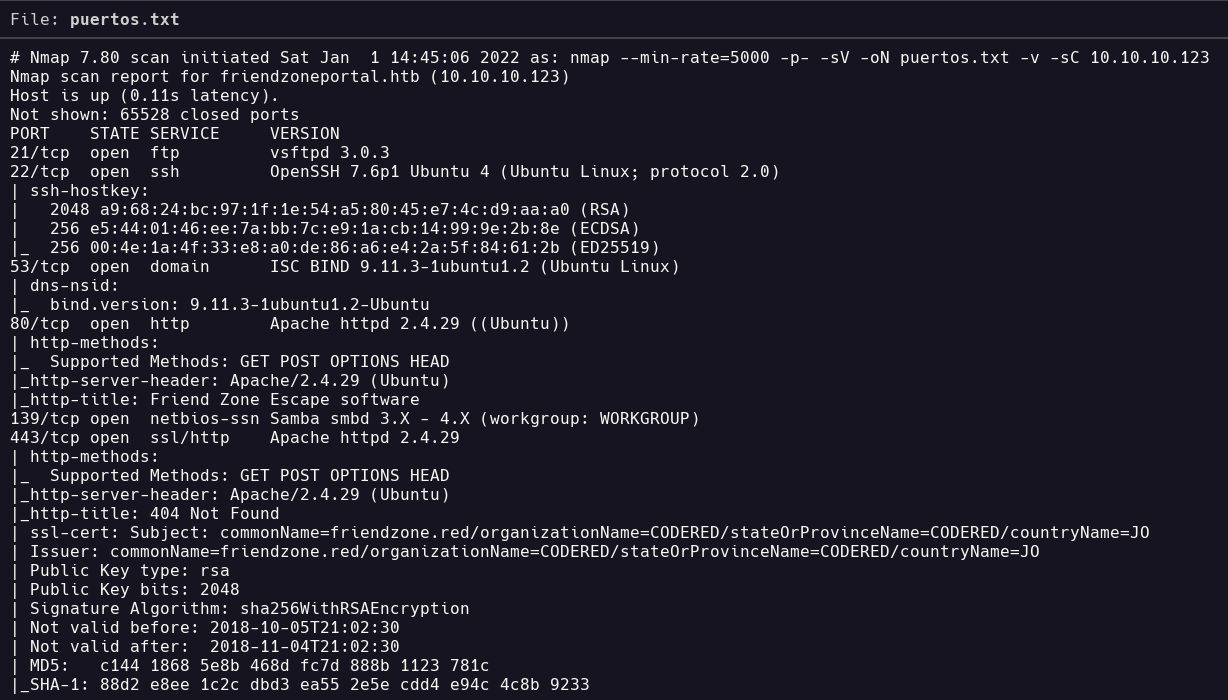
\includegraphics[width=\textwidth]{images/friendzone/puertos-nmap.png}
	\caption{escaneo con nmap}
\end{figure}
Encontramos el puerto 80 y el 443 abiertos, pero este último aparece con un nombre de dominio específico, así que vamos a darle un vistazo.
\begin{figure}[H]
	\center
	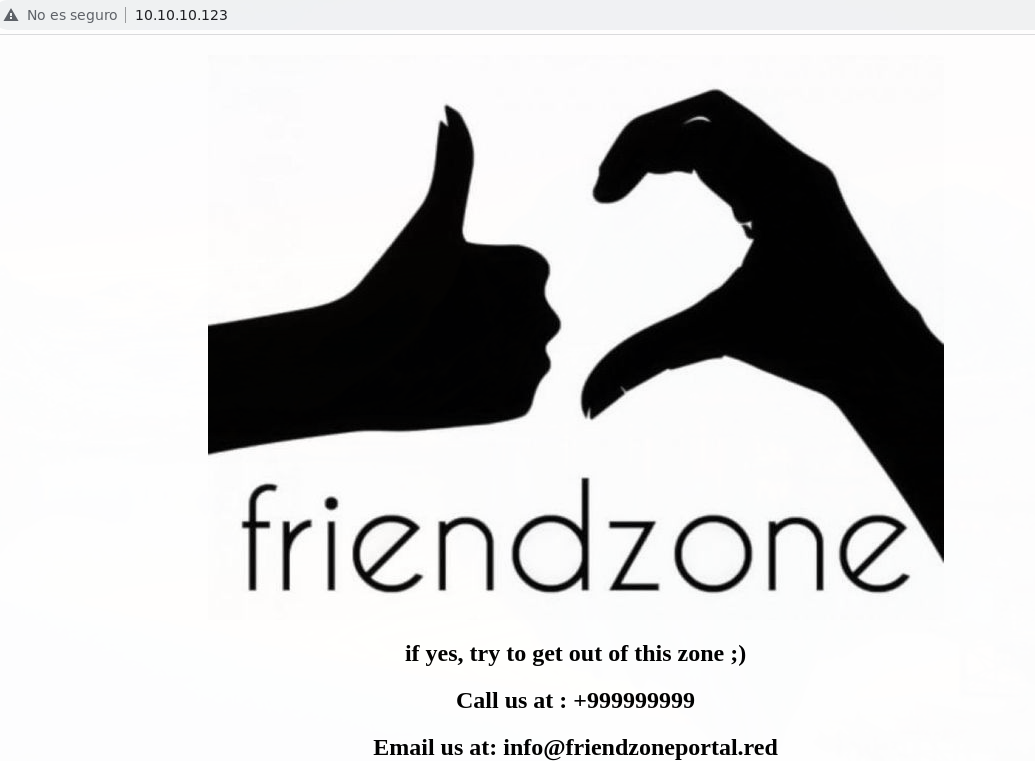
\includegraphics[width=\textwidth]{images/friendzone/puerto80.png}
	\caption{página del puerto 80}
\end{figure}
Para poder mostrar la página del 443 necesitamos primero modificar el /etc/hosts y añadirle el dominio que sale en el escaneo que es "friendzone.red".
Pero al hacer eso vemos que tiene otra página, entonces ya sabemos que es un vhost y para hallar el resto usaremos la técnica de transferencia de zona, "afxr".

\begin{figure}[H]
	\center
	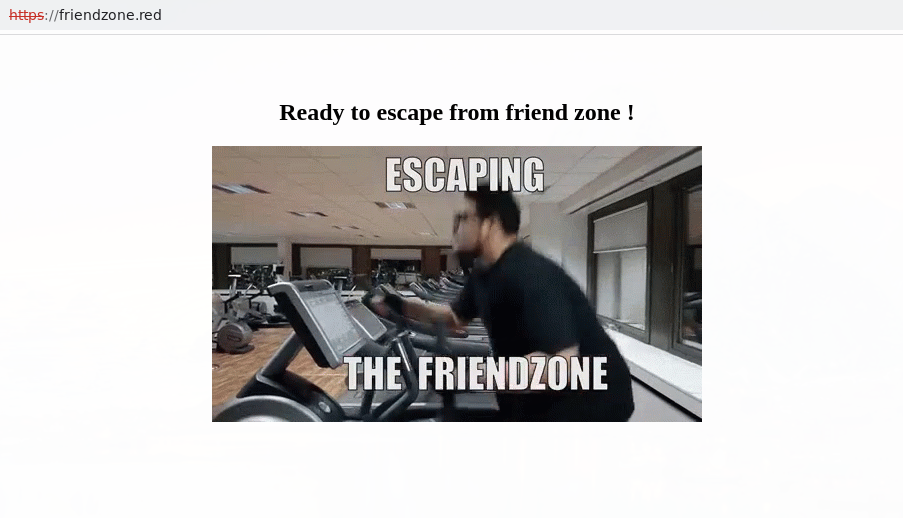
\includegraphics[width=\textwidth]{images/friendzone/puerto443.png}
	\caption{página del puerto 443}
\end{figure}

Necesitamos entonces usar el comando dig que es una utilidad que viene al instalar "dnsutils" junto con nslookup, luego de instalarlo y ejecutarlo con el parámetro axfr, nos muestra lo siguiente.

\begin{figure}[H]
	\center
	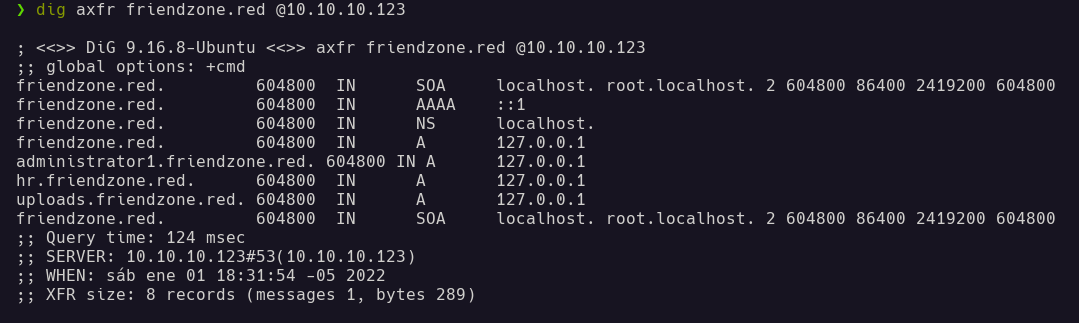
\includegraphics[width=\textwidth]{images/friendzone/dig-information.png}
	\caption{resultado ejecución dig}
\end{figure}



\begin{figure}[H]
	\center
	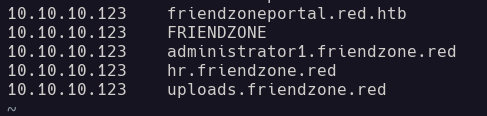
\includegraphics[width=\textwidth]{images/friendzone/modificacion-hosts.png}
	\caption{modificación /etc/hosts}
\end{figure}

Entonces dentro de estos vemos las páginas que están disponibles y encontramos las siguientes: 

\begin{itemize}
	\item hr.friendzone.red
	\item upload.friendzone.red
	\item administrator1.friendzone.red
\end{itemize}

Vimos que entrando a administrator1.friendzone.red encontramos un login, pero nos faltan las credenciales y no hemos tenido mucha información para obtenerla.
por lo que tocó investigar un poco los otros puertos, y descubrimos el puerto samba en el 445.

\begin{figure}[H]
	\center
	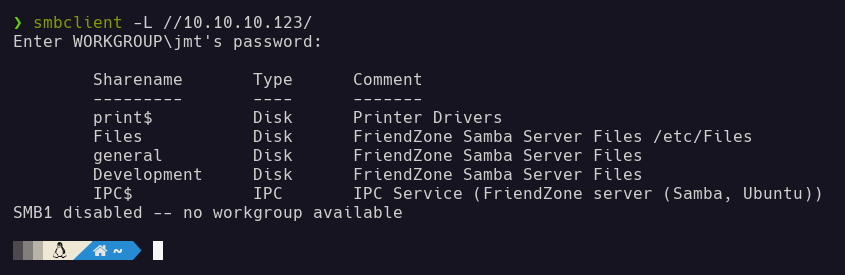
\includegraphics[width=\textwidth]{images/friendzone/samba-escaneo.png}
	\caption{listado de directorios en samba}
\end{figure}

Tenemos algunos directorios enumerados, pero solo tenemos permiso de lectura y escritura en dos, en "general" y "Development", algo que nos llama la atención es que "Files" es referenciado como "/etc/Files", los cual podría indicar una subida directa al /etc.


\begin{figure}[H]
	\center
	\includegraphics[width=\textwidth]{images/friendzone/conexión-general-samba.png}
	\caption{acceso a "general"}
\end{figure}

Pero más interesante lo que encontramos dentro, fue un "creds.txt" lo cual suena muy prometedor sin embargo, no lo podemos ver directamente.

\begin{figure}[H]
	\center
	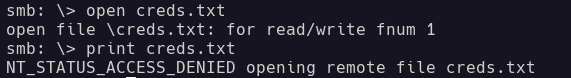
\includegraphics[width=\textwidth]{images/friendzone/intento-lectura-samba.png}
	\caption{intento de lectura}
\end{figure}

Entonces lo descargamos con el comando "get" del smbclient, y una vez descargado ya lo podremos leer.
Una vez descargado vimos que contiene credenciales de lo que parece un usuario administrador.

\begin{figure}[H]
	\center
	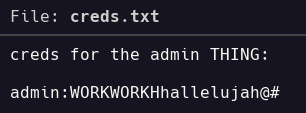
\includegraphics[width=\textwidth]{images/friendzone/cat-creds.png}
	\caption{lectura creds.txt}
\end{figure}

Probamos entonces con el ftp a ver si tenemos suerte, pero no obtuvimos nada.

\begin{figure}[H]
	\center
	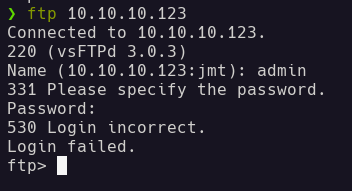
\includegraphics[width=\textwidth]{images/friendzone/login-ftp-fallido.png}
	\caption{fallo login ftp}
\end{figure}

Pero nos dimos cuenta que realmente las credenciales eran de la página de login en "administrator1.friendzone.red"

\begin{figure}[H]
	\center
	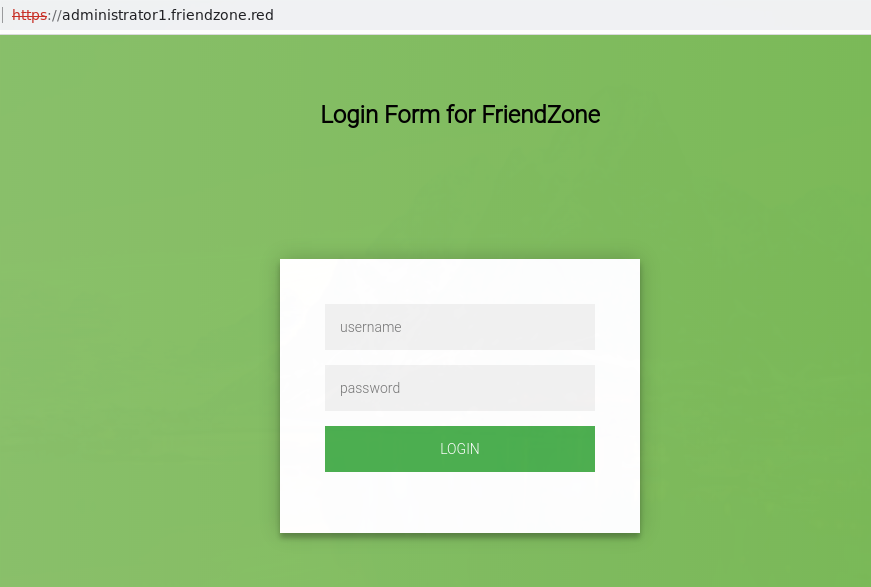
\includegraphics[width=\textwidth]{images/friendzone/login-administrator.png}
	\caption{fallo login ftp}
\end{figure}

Una vez logueados vemos que nos dice que nos redirigamos a "dashboard.php"

\begin{figure}[H]
	\center
	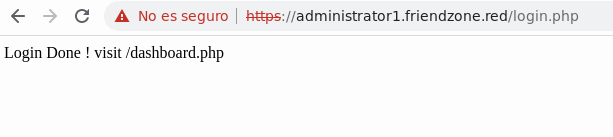
\includegraphics[width=\textwidth]{images/friendzone/login-correcto.png}
	\caption{fallo login ftp}
\end{figure}

\subsection{Explotación}

Dentro del dashboard nos dan instrucciones de cómo deberíamos redirigirnos a la imagen apuntando a un timestamp para controlar, vemos que este timestamp es una página eh php que ejecuta el servidor cada vez que apuntas a él, esto lo sabemos gracias a un escaneo de directorios a la ruta "administrator1.friendzone.red"

Entonces podemos subir una página php que ejecute una reverse shell y apuntar a esta en lugar del timestamp, pero para subir esta página hay dos formas:
\begin{itemize}
	\item usando el "upload.friendzone.red".
	\item subiendo por samba a un directorio que permita escritura.
\end{itemize}

Tuve un problema con el upload.friendzone.red ya que había realizado demasiadas consultas, así que intenté con la otra forma.

\begin{figure}[H]
	\center
	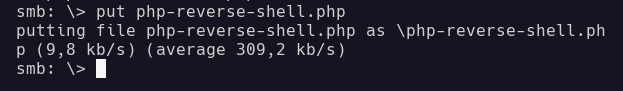
\includegraphics[width=\textwidth]{images/friendzone/subiendo-reverse.png}
	\caption{subiendo mediante samba la reverse shell}
\end{figure}

Esta reverse shell la pueden encontrar del siguiente github: "https://github.com/d4t4s3c/Offensive-Reverse-Shell-Cheat-Sheet".

Entonces solo quedaría correr un nmap en escucha con el comando "nmap -lvnp 1234".
y luego ejecutar la ejecución en la página.

\begin{figure}[H]
	\center
	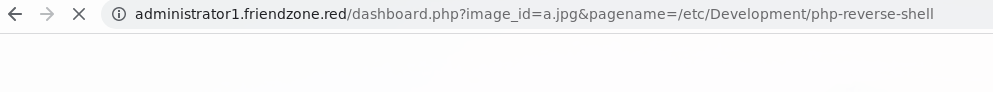
\includegraphics[width=\textwidth]{images/friendzone/ejecucion-reverse.png}
	\caption{ejecutando la reverse shell}
\end{figure}

y obtenemos la conexión luego de esto.

\begin{figure}[H]
	\center
	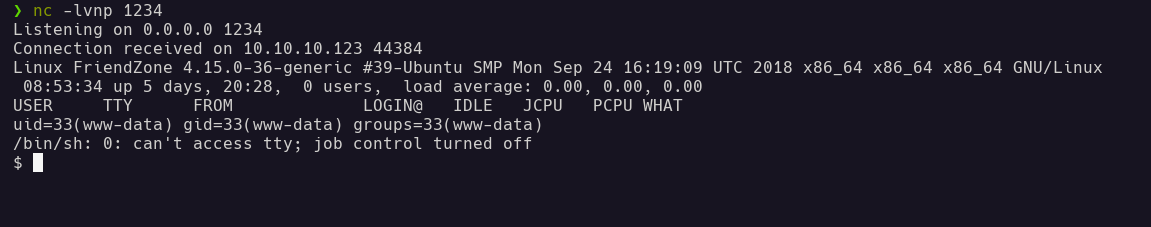
\includegraphics[width=\textwidth]{images/friendzone/shell-obtenida.png}
	\caption{obtención de shell}
\end{figure}

Ya con esto es suficiente para leer el "user.txt" del usuario friendzone, lo cual es un poco raro porque solo somos www-data cuando entramos al dispositivo.

\begin{figure}[H]
	\center
	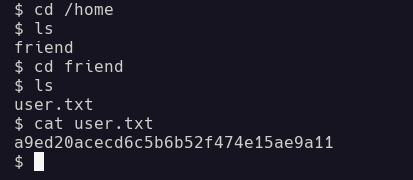
\includegraphics[width=\textwidth]{images/friendzone/flag-user.png}
	\caption{flag del user friendzone}
\end{figure}


\subsection{Escalamiento de privilegios}

% ----------------------------Omni-----------------------------------
\clearpage 
\section{Omni}
\subsection{Enumeración}
Primero se realizó un escaneo de los puertos abiertos con Nmap, con los parámetros “-Pn -A -p-“.
\begin{figure}[H]
	\center
	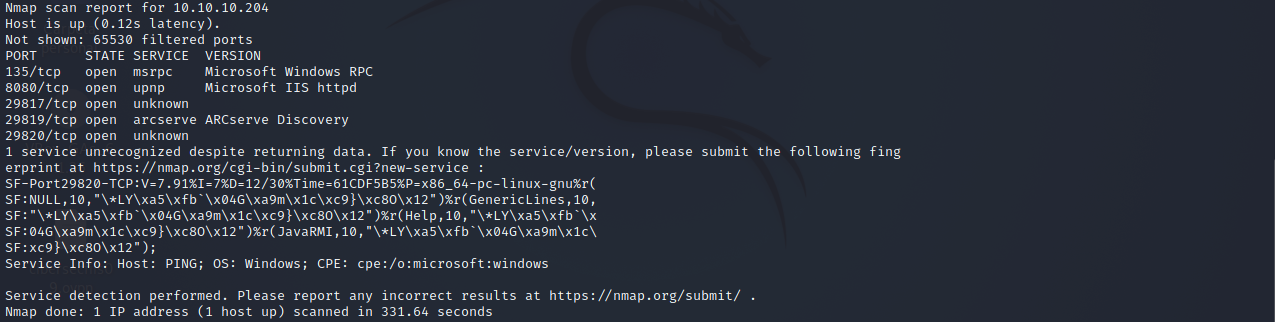
\includegraphics[width=\textwidth]{images/omni/1.png}
	\caption{Escaneo de Puertos}
\end{figure}

Se llegó a encontrar 5 puertos abiertos, los cuales el 135 y 8080 nos llama la atención. En el puerto 135 está corriendo el servicio de Microsoft Windows RPC (msrpc) y en el 8080 Microsoft IIS http (npnp), el cual es un servicio web. El servicio msrpc implementa el protocolo RPC, una forma de comunicación entre procesos de bajo nivel en la que un proceso de cliente puede realizar solicitudes de un proceso de servidor.  Probamos conectarnos con rpcclient de forma anónima pero no permite.
\begin{figure}[H]
	\center
	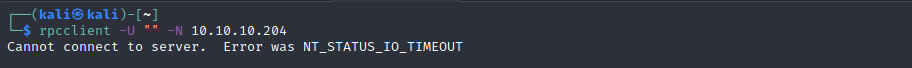
\includegraphics[width=\textwidth]{images/omni/2.png}
	\caption{RPCCLIENT}
\end{figure}

Por lo que accedemos mediante el navegador al 10.10.10.204:8080 y nos arroja una ventana que nos pide autenticarnos para “Windows Device Portal”.
\begin{figure}[H]
	\center
	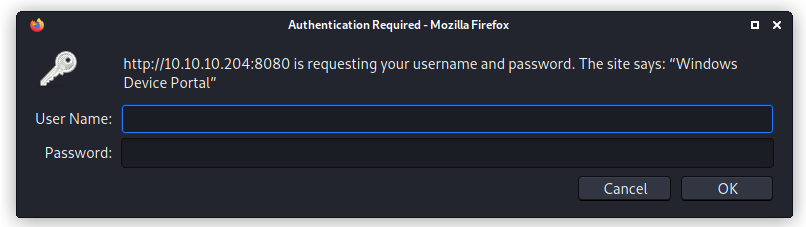
\includegraphics[width=\textwidth]{images/omni/3.png}
	\caption{Autenticación 10.10.10.204:8080}
\end{figure}

\subsection{Explotación}

Según la documentación de Microsoft, Windows Device Portal o Portal de dispositivos Windows (WDP) es un servidor web que se incluye con los dispositivos Windows, y que le permite configurar y administrar la configuración del dispositivo a través de una red o una conexión USB (también se admiten conexiones locales en dispositivos con un explorador web).
Buscando vulnerabilidades y exploits del WDP nos encontramos con SirepRAT (\href{https://github.com/SafeBreach-Labs/SirepRAT}), el cual es una vulnerabilidad del servicio de Sirep Test y expone la ejecución de comandos de forma remota. Mediante esto nos permite descargar archivos de la máquina víctima, subir archivos, correr programas, obtener información del sistema y obtener información de archivos.

En este caso subiremos un archivo, específicamente netcat (\href{https://github.com/int0x33/nc.exe/}) para lograr una reverse Shell en nuestra máquina.
Para lograr esto se levantó un servidor simplehttp con Python y mediante la opción de ejecutar comandos utilizamos powershell (\href{https://academy.hackthebox.com/course/preview/file-transfers/windows-file-transfer-methods}) para descargar el binario.
Primero se probó con la versión de 32 bits, pero nos arroja error que se solucionó utilizando la de 64 bits.
\begin{figure}[H]
	\center
	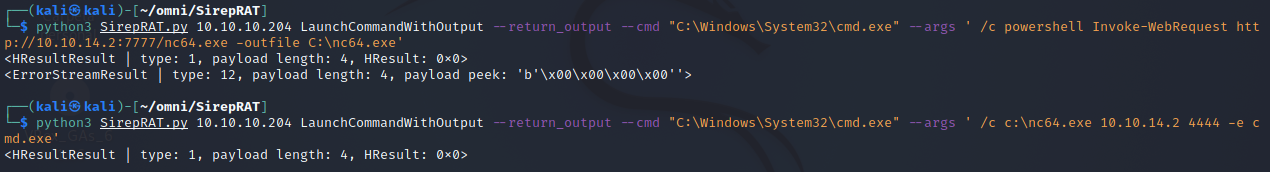
\includegraphics[width=\textwidth]{images/omni/5.png}
	\caption{Descarga del nc64.exe}
\end{figure}

Pero antes de ejecutar el netcat debemos levantar en nuestra máquina el servicio netcat con un puerto en modo escucha que debe de coincidir con el comando que se ejecutará en la máquina victima con el nc.exe.
\begin{figure}[H]
	\center
	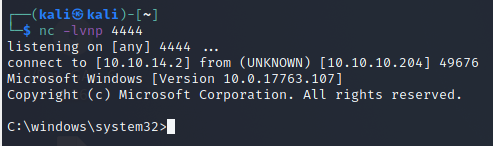
\includegraphics[width=\textwidth]{images/omni/6.png}
	\caption{Netcat en modo de escucha}
\end{figure}
\begin{figure}[H]
	\center
	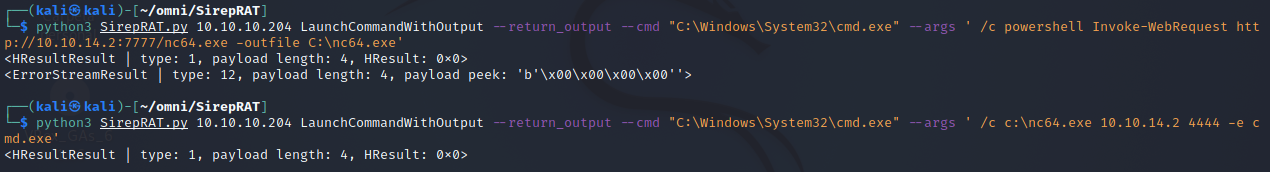
\includegraphics[width=\textwidth]{images/omni/7.png}
	\caption{Ejecución del nc64.exe}
\end{figure}

Y listo, tenemos acceso a la máquina, pero somos el usuario “omni”.
\begin{figure}[H]
	\center
	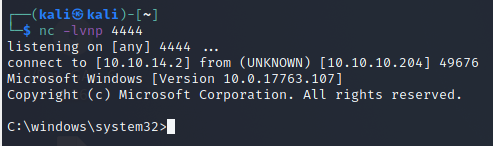
\includegraphics[width=\textwidth]{images/omni/8.png}
	\caption{Acceso obtenido en el netcat}
\end{figure}

Inspeccionando los archivos encontramos el archivo flag “user.txt” pero al ver su contenido se vió lo siguiente, un archivo PSCredential. Los archivos PSCredential son generados cuando se encripta información sensible mediante PowerShell, pero para poder recuperar esto es necesario estar logeado con el usuario dueño.
\begin{figure}[H]
	\center
	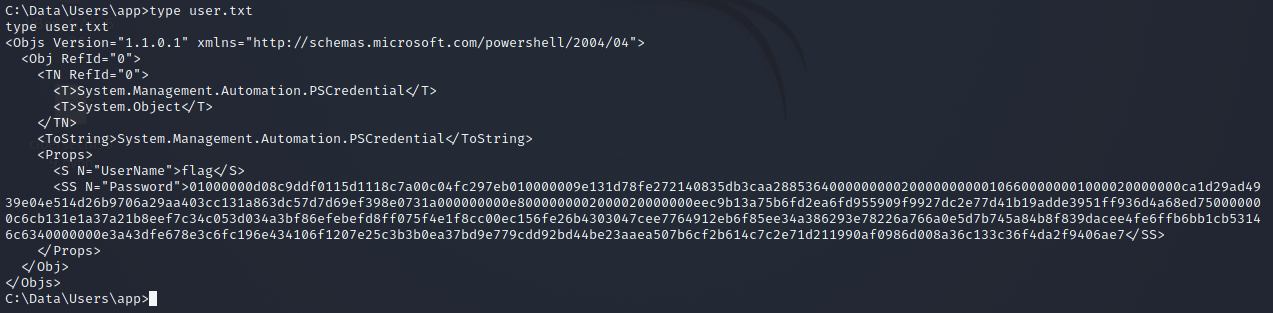
\includegraphics[width=\textwidth]{images/omni/9.png}
	\caption{user.txt}
\end{figure}

Para ello necesitamos tener las credenciales del usuario, esto lo podemos hacer dumpeando los archivos .hiv de system, sam y security, y luego mediante secretsdump.py obtener los hashes de las credenciales.
Primero levantaremos un servidor Samba en nuestra máquina mediante smbserver.py para copiar estos archivos requeridos. La máquina víctima nos pide usar el protocolo SMB2, esto lo arreglamos añadiendo la opción de -smb2support a la hora de correr el smbserver.py además añadimos credenciales. (https://pure.security/dumping-windows-credentials/)
\begin{figure}[H]
	\center
	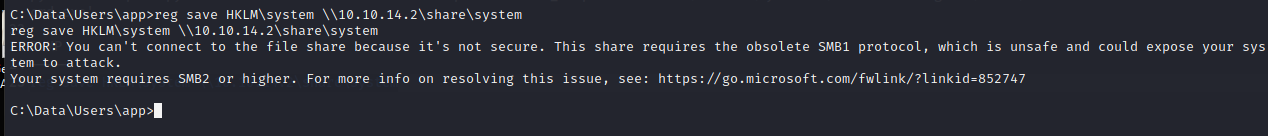
\includegraphics[width=\textwidth]{images/omni/10.png}
	\caption{Error de conexión al SMB1}
\end{figure}
\begin{figure}[H]
	\center
	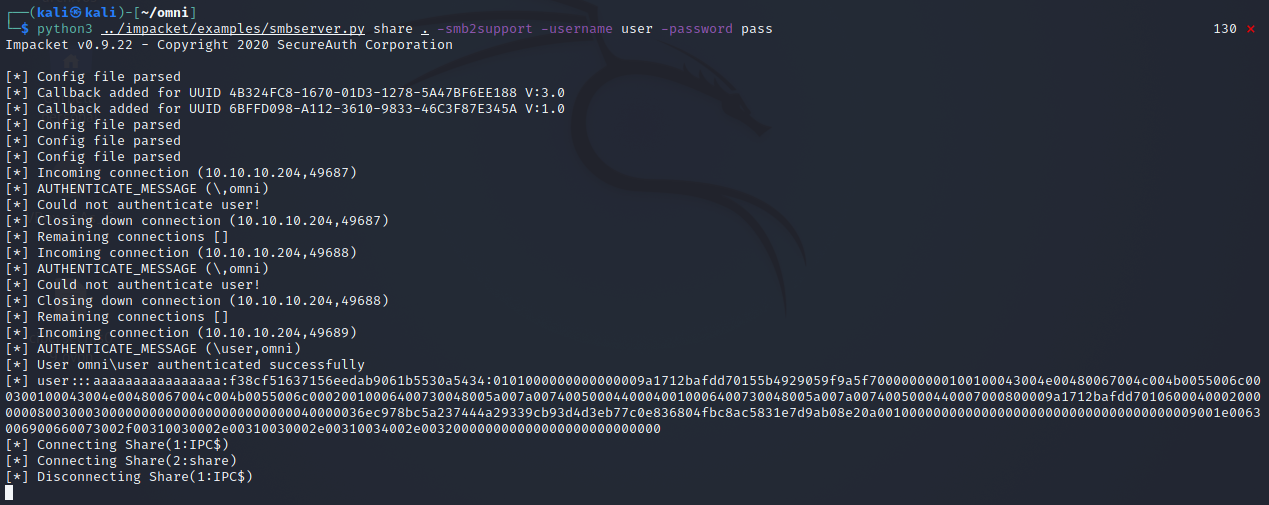
\includegraphics[width=\textwidth]{images/omni/11.png}
	\caption{Arreglo con soporte al SMB2 y autenticación}
\end{figure}

Montamos la carpeta compartida mediante el smbserver.py y procederemos a copiar los archivos .hiv hacia ahí.
\begin{figure}[H]
	\center
	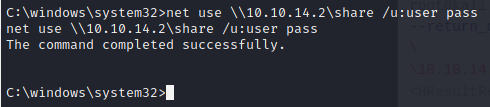
\includegraphics[width=\textwidth]{images/omni/12.png}
	\caption{Montado de la carpeta compartida}
\end{figure}
\begin{figure}[H]
	\center
	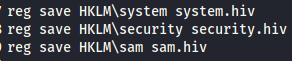
\includegraphics[width=\textwidth]{images/omni/13.png}
	\caption{Extracción de los hives}
\end{figure}
\begin{figure}[H]
	\center
	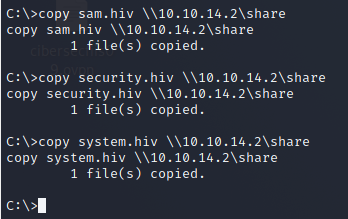
\includegraphics[width=\textwidth]{images/omni/14.png}
	\caption{Copiado de los hives a la carpeta compartida}
\end{figure}

Una vez copiado utilizamos secretsdump.py para obtener los hashes.
\begin{figure}[H]
	\center
	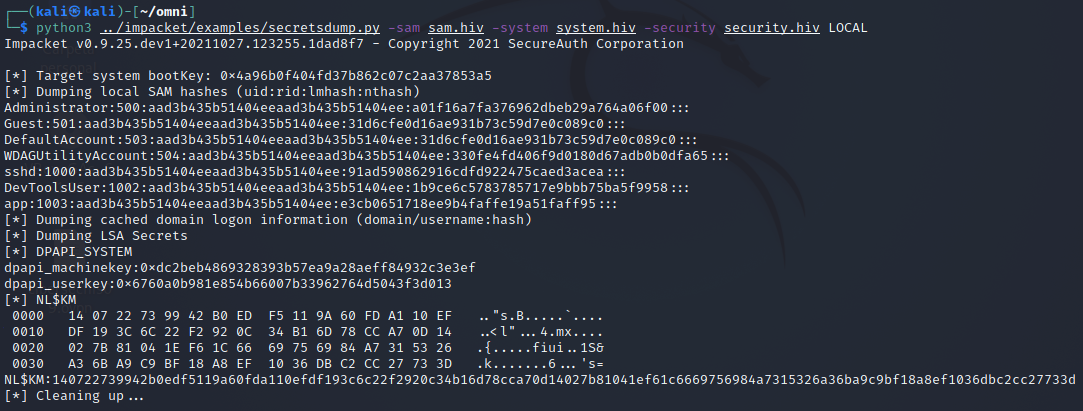
\includegraphics[width=\textwidth]{images/omni/15.png}
	\caption{Obtención de los hashes con secretsdump.py}
\end{figure}

Una vez obtenido los hashes lo copiamos a un archivo, en este caso llamando “hashes” y con JohnTheRipper (john) procederemos a crackearlo.
\begin{figure}[H]
	\center
	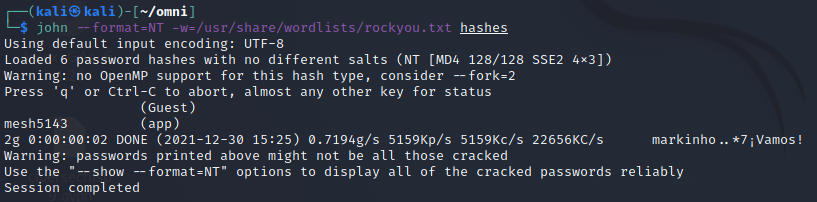
\includegraphics[width=\textwidth]{images/omni/16.png}
	\caption{Crackeo del hash con JohnTheRipper (john)}
\end{figure}

Nos arroja que para el usuario app su contraseña es “mesh5143”. Con estas credenciales podemos acceder al WDP.
\begin{figure}[H]
	\center
	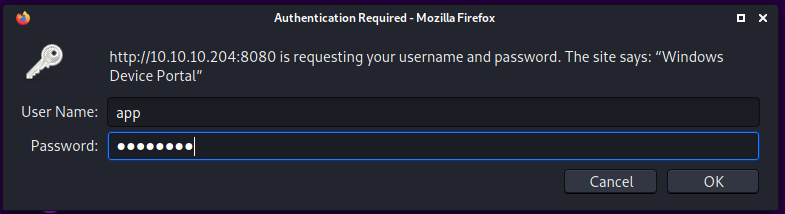
\includegraphics[width=\textwidth]{images/omni/17.png}
	\caption{Autenticación con los credenciales del usuario app}
\end{figure}

Una vez dentro nos encontramos en la pantalla principal del WDP donde nos permite manejar y administrar el dispositivo IoT.
\begin{figure}[H]
	\center
	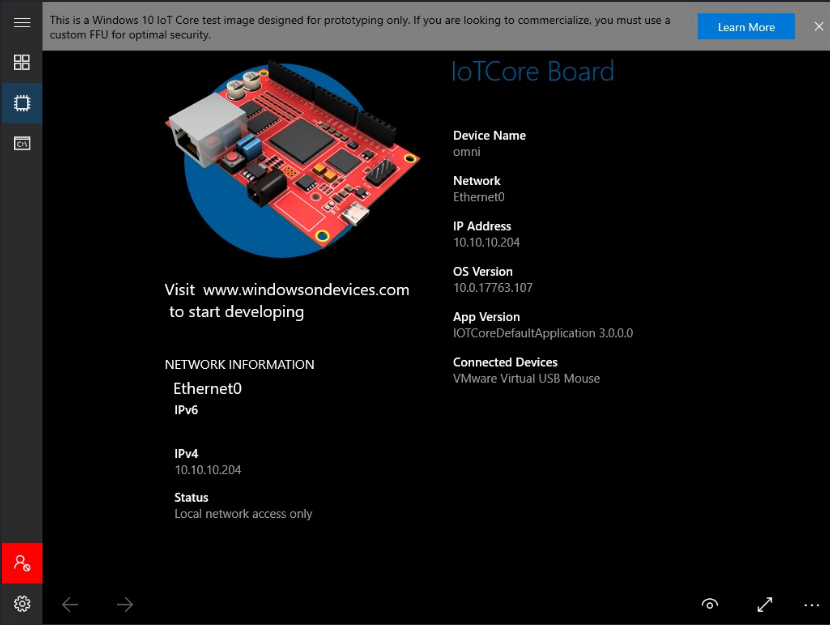
\includegraphics[width=0.8\textwidth]{images/omni/18.png}
	\caption{Screenshot de la pantalla del dispositivo IoT}
\end{figure}
\begin{figure}[H]
	\center
	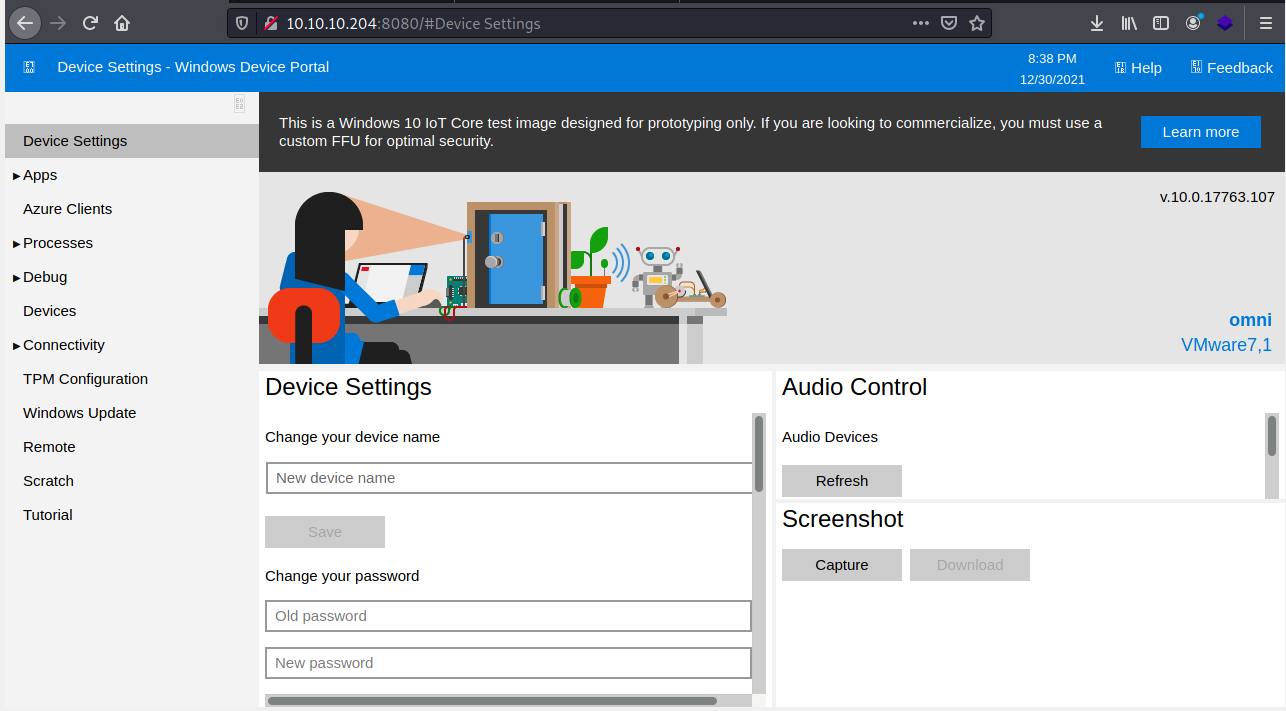
\includegraphics[width=\textwidth]{images/omni/19.png}
	\caption{Pantalla principal del WDP}
\end{figure}
\begin{figure}[H]
	\center
	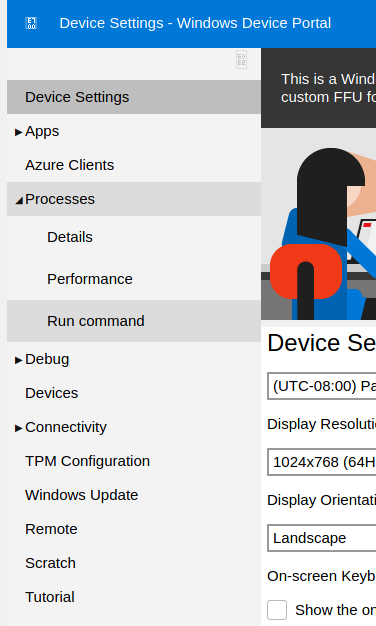
\includegraphics[width=0.3\textwidth]{images/omni/20.png}
	\caption{Opciones del WDP}
\end{figure}

Una vez dentro en la categoría de Procesos vemos una opción para ejecutar comandos, con esto podemos obtener una reverse Shell del usuario “app”. Para ello levantaremos el netcat en modo escucha y ejecutamos los mismos comandos anteriormente.
\begin{figure}[H]
	\center
	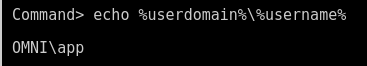
\includegraphics[width=0.7\textwidth]{images/omni/21.png}
	\caption{Usuario app}
\end{figure}
\begin{figure}[H]
	\center
	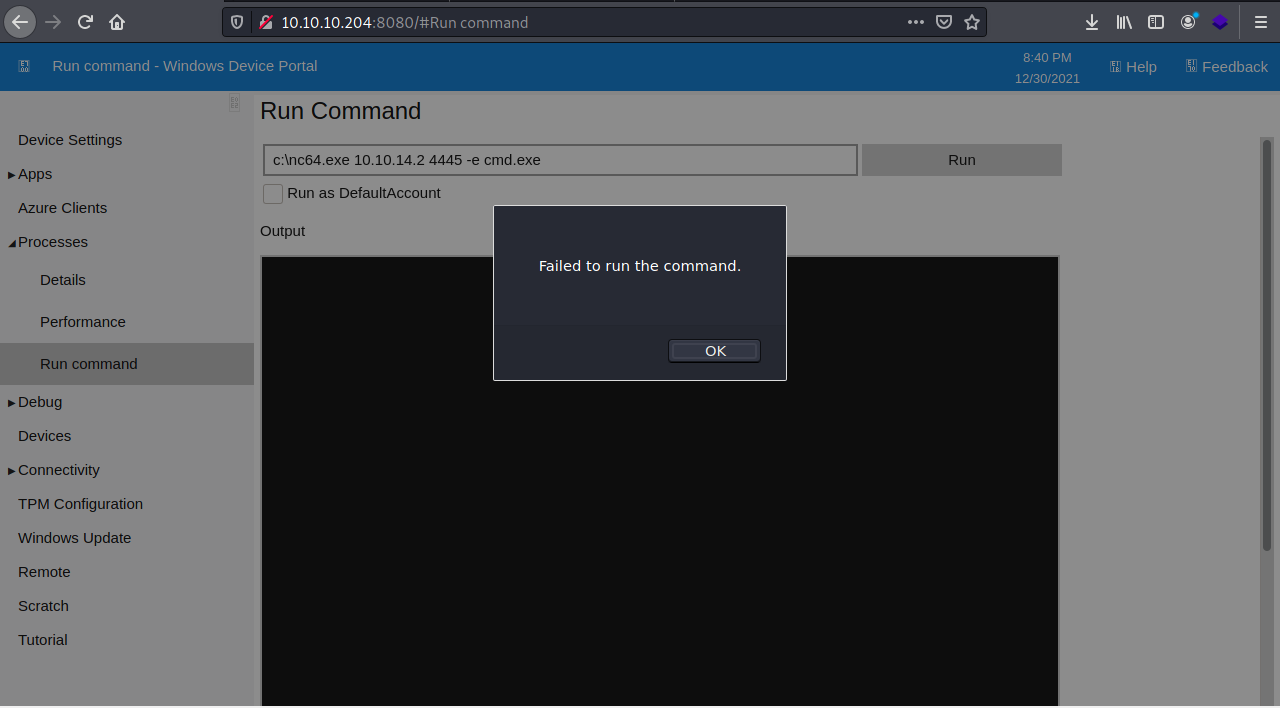
\includegraphics[width=\textwidth]{images/omni/22.png}
	\caption{Mensaje de error de ejecución del comando}
\end{figure}

A pesar que nos bota error que falló en ejecutar el comando, en el terminal podemos ver que ya se estableció conexión y ya tenemos acceso mediante el usuario “app”.
\begin{figure}[H]
	\center
	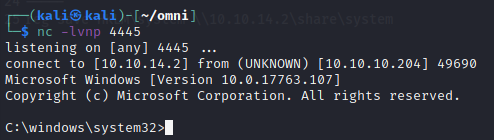
\includegraphics[width=0.9\textwidth]{images/omni/23.png}
	\caption{Conexión establecida}
\end{figure}

Con el acceso podremos recuperar la información del archivo PSCredential mediante PowerShell y Import-CliXml.
\begin{figure}[H]
	\center
	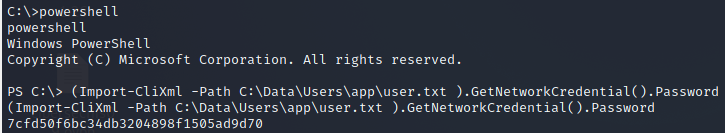
\includegraphics[width=\textwidth]{images/omni/24.png}
	\caption{Obtención de la flag en user.txt}
\end{figure}

Y listo tenemos la flag del user.txt. Inspeccionando los demás archivos que se encuentran en la misma carpeta destaca “hardening.txt” y “iot-admin.xml”.
\begin{figure}[H]
	\center
	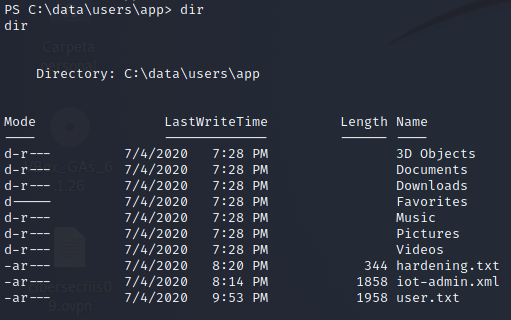
\includegraphics[width=0.8\textwidth]{images/omni/25.png}
	\caption{Directorio del usuario app}
\end{figure}

\subsection{Escalamiento de privilegios}

Inspeccionando el contenido de ambos archivos vemos que en hardening está algunas acciones realizadas y el iot-admin.xml es otro archivo PSCredential, por lo que ejecutamos el mismo comando anterior y obtendremos la contraseña, el cual resulta ser la contraseña del usuario administrator para ser utilizado en el WDP.
\begin{figure}[H]
	\center
	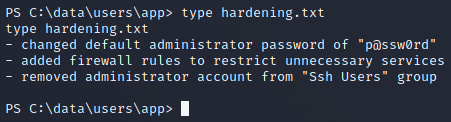
\includegraphics[width=\textwidth]{images/omni/26.png}
	\caption{Archivo hardening.txt}
\end{figure}
\begin{figure}[H]
	\center
	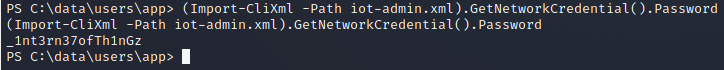
\includegraphics[width=\textwidth]{images/omni/27.png}
	\caption{Flag del iot-admin.xml}
\end{figure}

Hacemos lo mismo realizado para lograr una reverse Shell mediante el usuario “app“ pero ahora como administrator.
\begin{figure}[H]
	\center
	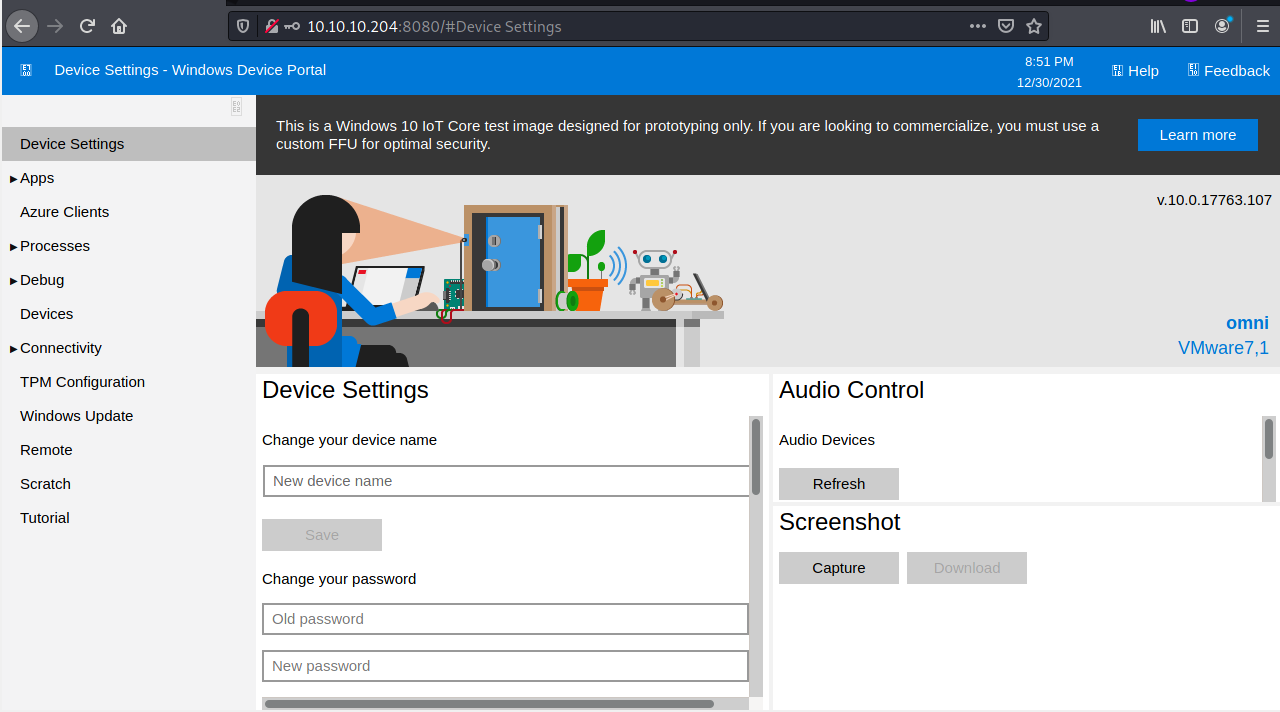
\includegraphics[width=\textwidth]{images/omni/28.png}
	\caption{Pantalla principal del WDP del usuario administrator}
\end{figure}
\begin{figure}[H]
	\center
	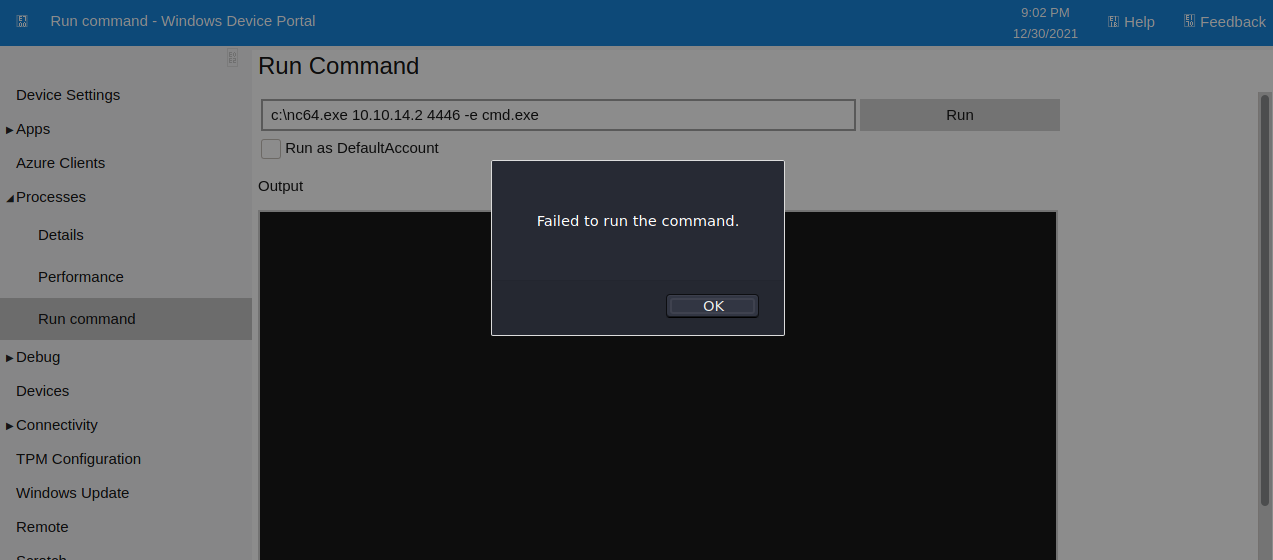
\includegraphics[width=\textwidth]{images/omni/29.png}
	\caption{Mensaje de error de ejecución del comando}
\end{figure}
\begin{figure}[H]
	\center
	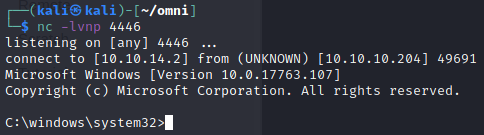
\includegraphics[width=\textwidth]{images/omni/30.png}
	\caption{Establecimiento de la conexión}
\end{figure}
\begin{figure}[H]
	\center
	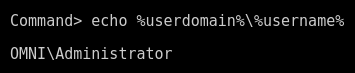
\includegraphics[width=0.9\textwidth]{images/omni/31.png}
	\caption{Usuario administrator}
\end{figure}

Y listo, tenemos acceso como el usuario administrator, ahora solo queda abrir el archivo root.txt, el cual es otro archivo PSCredential y con el mismo comando tendremos su contraseña o flag en este caso.
\begin{figure}[H]
	\center
	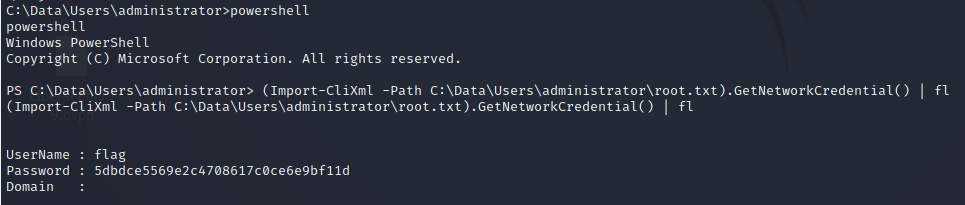
\includegraphics[width=\textwidth]{images/omni/32.png}
	\caption{Flag del root.txt}
\end{figure}

\end{document}
